\chapter{Evaluation}
\label{ch:evaluation}

After we finished implementing our system, we began to evaluate our system
in terms of performances of response speed and memory usage. To evaluate
the system, we need some decent amount of sample data, so here we
introduce the standard name list.

\section{Introducing standard name list}
\label{sec:stdname}

In subsection \ref{sub:lookuptable}, we mentioned Robert Edwin Matheson,
who developed a classification of Irish names. He classified
the surnames in Ireland into 2091 groups. Adam Winstanley's work
on this classification \cite[]{adamw} looked through these groups
and came up with a total 12,944 names in this classification.
We use all these names to build up our lookup table (section \ref{sec:lookuptable}).

We also decide to use all these records as a standard name list,
for example, a client may want to match the \emph{base name} `MONAHAN'
for all any possible matching \emph{to-match names}. A client has
an option to choose to match `MONAHAN' with all 12,944 names in
our standard list.

For web service clients, specify \texttt{standard\_list} as
\texttt{true}, \texttt{t}, or \texttt{1} to use the standard list.
For example in listing \ref{lst:json_std}, note that
\texttt{to\_match\_names} is left blank and \texttt{standard\_list} value is 1.

\begin{minipage}{\linewidth}
  \begin{lstlisting}[language={json}, label={lst:json_std}, caption={Sample \texttt{JSON} with a standard name list option.}]
{
  "base_names":"Monahan",
  "to_match_names":"",
  "matching_algorithms":{
    "1":{"name":"LookupTable", "weight":"10"},
    "2":{"name":"LevenshteinDistance", "weight":"1"},
    "3":{"name":"Soundex", "weight":"3"},
    "4":{"name":"IrishSoundex", "weight":"6"}
  },
  "threshold":"0",
  "standard_list":"1"
}
\end{lstlisting}
\end{minipage}

For web interface clients, check the ``Use standard list'' checkbox
to use the standard list, as shown in figure \ref{fig:wi_std}.

\begin{figure}[H]
\centering
\captionsetup{justification=centering}
\makebox[\textwidth][c]{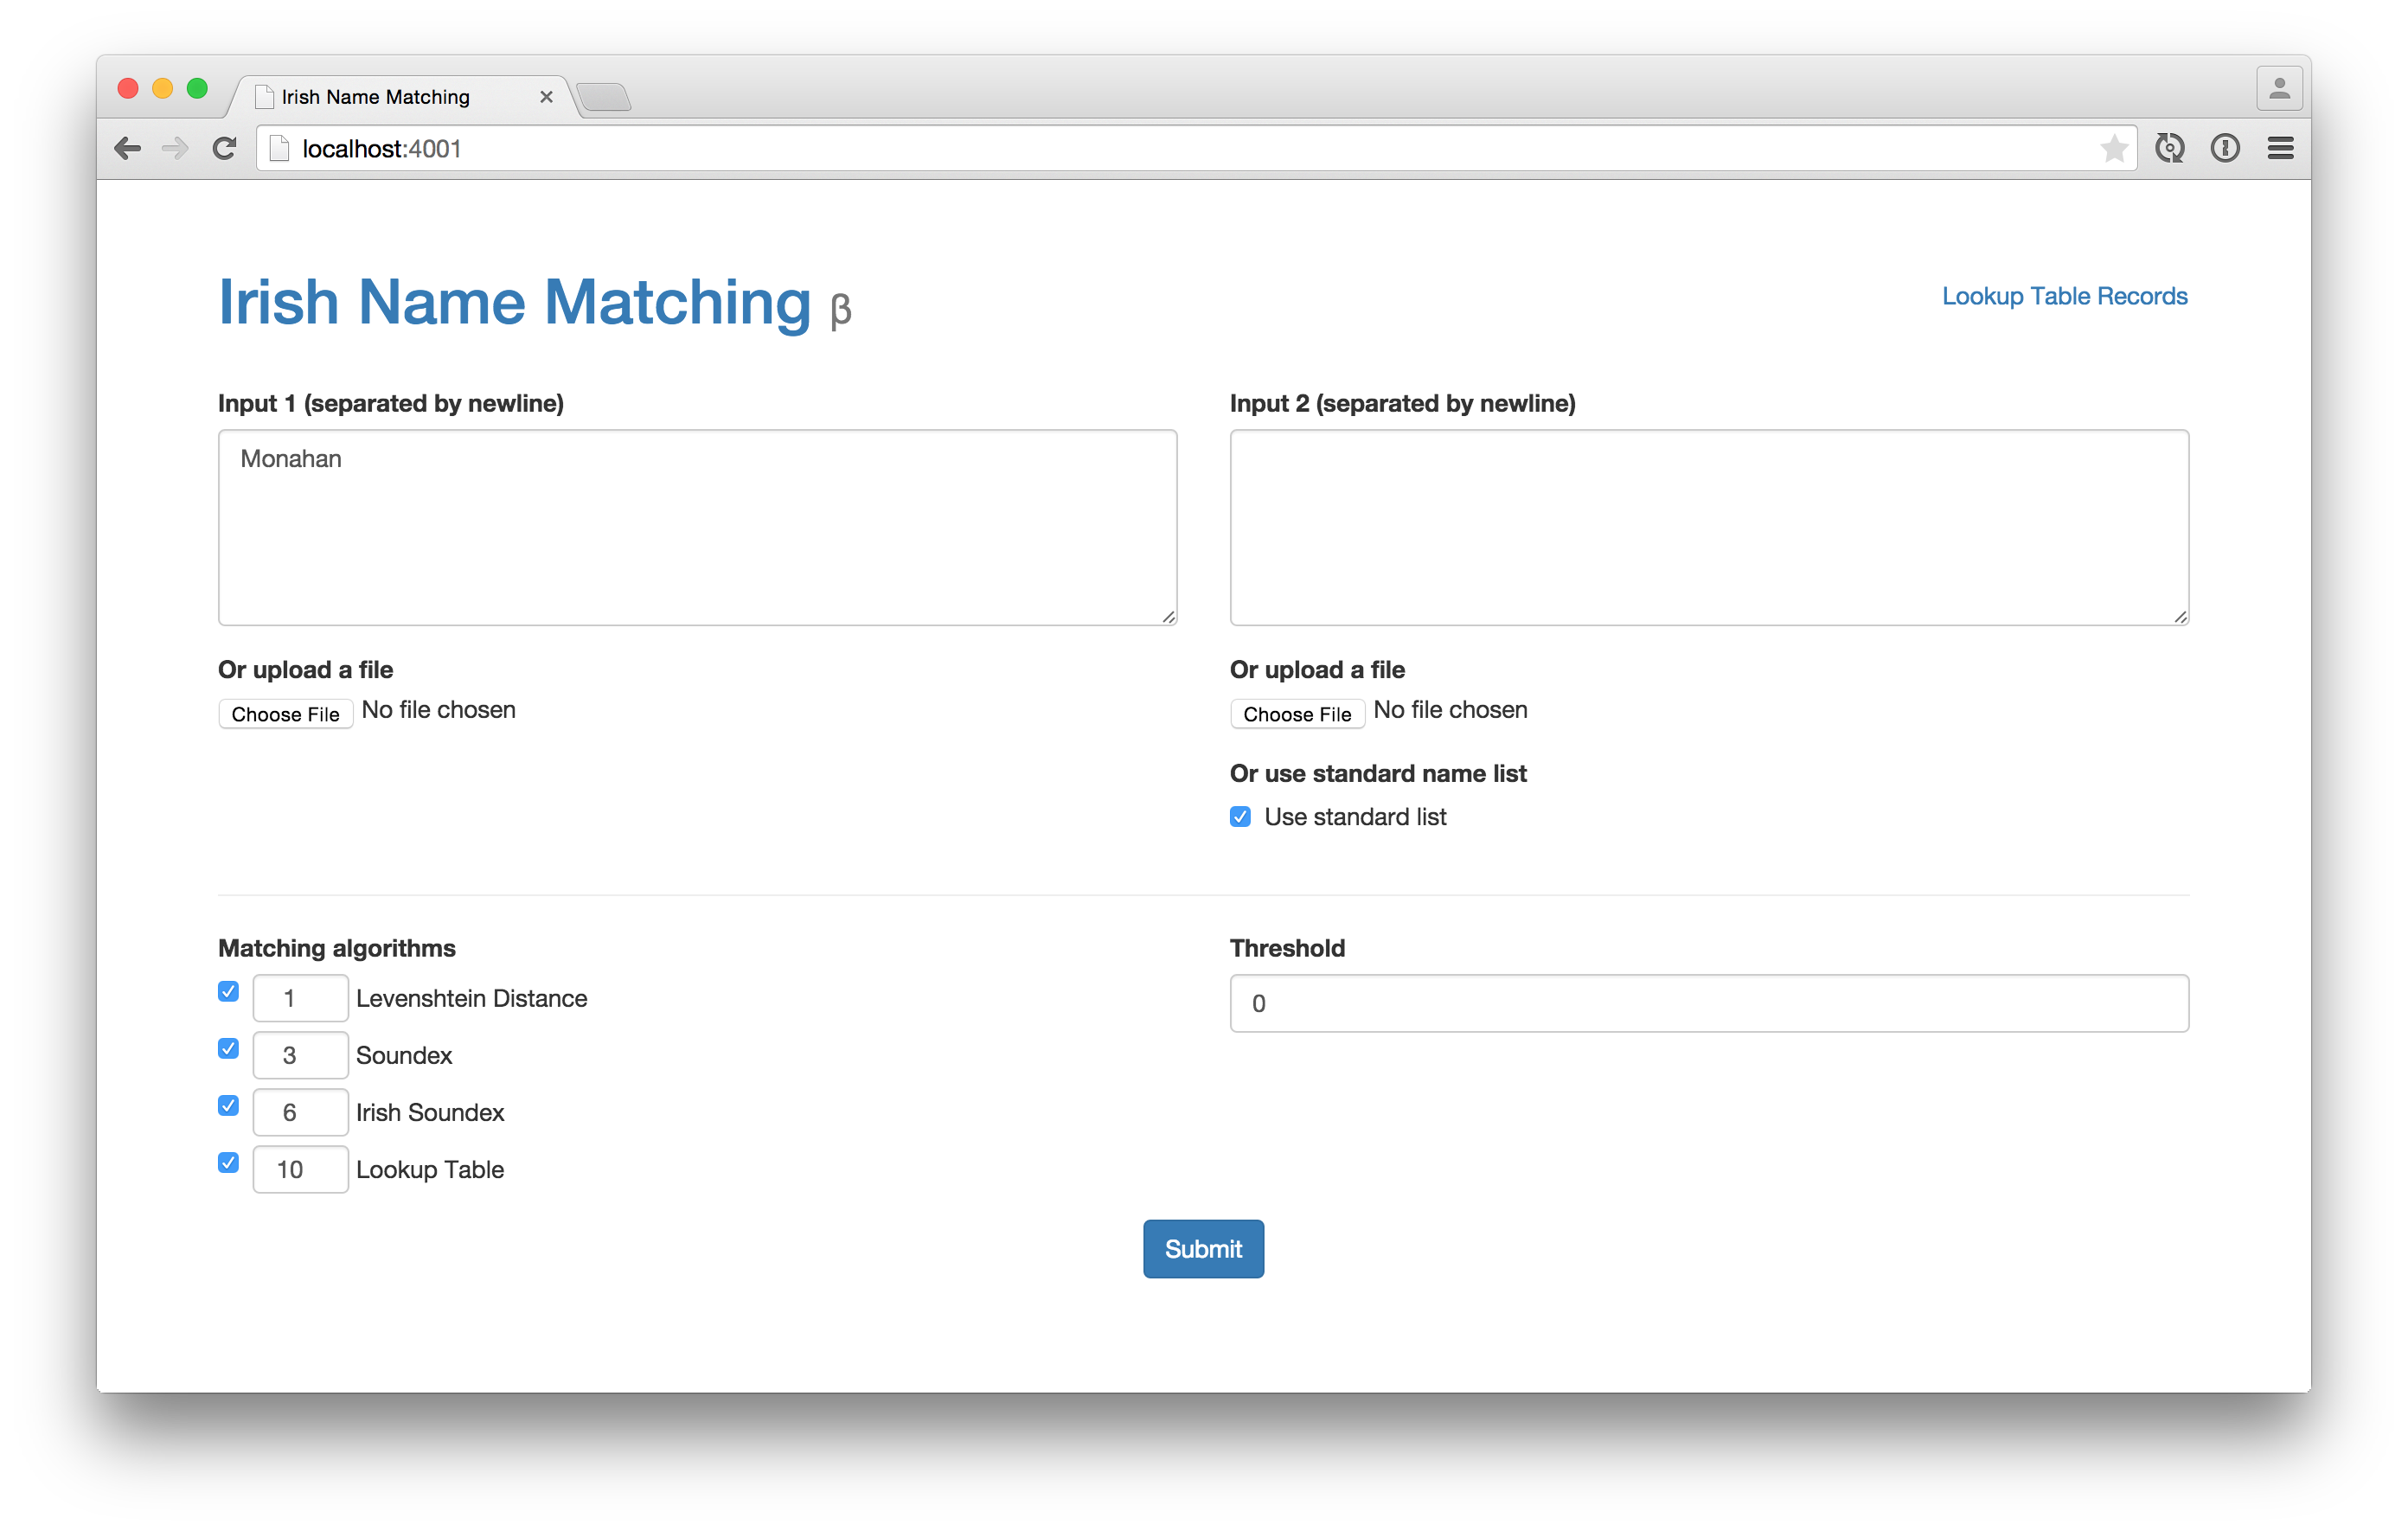
\includegraphics[width=16cm]{gfx/wi_std}}
\caption{Web interface with a standard name list option.}
\label{fig:wi_std}
\end{figure}

Using a standard name list option generates many results.
Client is suggested also specify a proper threshold (section \ref{sec:threshold})
to discard irreverent results.

In listing \ref{lst:json_std_out} is a result of matching between
\emph{base name} `MONAHAN' and the standard name list, using threshold as 0.9.
Results' detailed scores are truncated for readability.

\begin{minipage}{\linewidth}
  \begin{lstlisting}[language={json}, label={lst:json_std_out}, caption={Results of matching \emph{base name} `MONAHAN' with a standard name list.}]
[
  {
    "base_name": "MONAHAN",
    "to_match_names": [
      {
        "to_match_name": "MONAHAN",
        "overall_weighted_score": 1,
        ..
      },
      {
        "to_match_name": "MOYNAHAN",
        "overall_weighted_score": 0.994,
        ..
      },
      {
        "to_match_name": "MONOHAN",
        "overall_weighted_score": 0.993,
        ..
      },
      {
        "to_match_name": "MONEHAN",
        "overall_weighted_score": 0.993,
        ..
      },
      {
        "to_match_name": "MOYNIHAN",
        "overall_weighted_score": 0.988,
        ..
      },
      {
        "to_match_name": "MOYNAN",
        "overall_weighted_score": 0.979,
        ..
      }
    ]
  }
]
\end{lstlisting}
\end{minipage}

\section{Response speed}

\section{Memory usage}
